% !TEX TS-program = pdflatex
% !TEX encoding = UTF-8 Unicode

% This is a simple template for a LaTeX document using the "article" class.
% See "book", "report", "letter" for other types of document.

%\usepackage{extsizes}

%\documentclass[12pt]{article} % use larger type; default would be 10pt
\documentclass[14pt]{extarticle} % use larger type; default would be 10pt

\usepackage[utf8]{inputenc} % set input encoding (not needed with XeLaTeX)

%%% Examples of Article customizations
% These packages are optional, depending whether you want the features they provide.
% See the LaTeX Companion or other references for full information.

%%% PAGE DIMENSIONS
\usepackage{geometry} % to change the page dimensions
\geometry{a4paper} % or letterpaper (US) or a5paper or....
%\geometry{margin=2in} % for example, change the margins to 2 inches all round
%\geometry{left=2.75cm, right=2.75cm, top=3.5cm, bottom=4.5cm}
% \geometry{landscape} % set up the page for landscape
%   read geometry.pdf for detailed page layout information

\usepackage{graphicx} % support the \includegraphics command and options

% \usepackage[parfill]{parskip} % Activate to begin paragraphs with an empty line rather than an indent

%%% PACKAGES
\usepackage{booktabs} % for much better looking tables
\usepackage{array} % for better arrays (eg matrices) in maths
\usepackage{paralist} % very flexible & customisable lists (eg. enumerate/itemize, etc.)
\usepackage{verbatim} % adds environment for commenting out blocks of text & for better verbatim
\usepackage{subfig} % make it possible to include more than one captioned figure/table in a single float
% These packages are all incorporated in the memoir class to one degree or another...

%%% HEADERS & FOOTERS
\usepackage{fancyhdr} % This should be set AFTER setting up the page geometry
\pagestyle{fancy} % options: empty , plain , fancy
\renewcommand{\headrulewidth}{0pt} % customise the layout...
\lhead{}\chead{}\rhead{}
\lfoot{}\cfoot{\thepage}\rfoot{}

%%% SECTION TITLE APPEARANCE
%\usepackage{sectsty}
%\allsectionsfont{\sffamily\mdseries\upshape} % (See the fntguide.pdf for font help)
% (This matches ConTeXt defaults)

%%% ToC (table of contents) APPEARANCE
\usepackage[nottoc,notlof,notlot]{tocbibind} % Put the bibliography in the ToC
\usepackage[titles,subfigure]{tocloft} % Alter the style of the Table of Contents
\renewcommand{\cftsecfont}{\rmfamily\mdseries\upshape}
\renewcommand{\cftsecpagefont}{\rmfamily\mdseries\upshape} % No bold!

%%% BibTex packages (url for website references)
\usepackage[english]{babel}
\usepackage[round]{natbib}
% \usepackage{url}
% \usepackage{Biblatex}

%For inclusion of hyperlinks
\usepackage{hyperref}
\hypersetup{
	colorlinks=true,
	linkcolor=blue,
	filecolor=magenta,      
	urlcolor=cyan,
}

%BibTex stuff and referencing sections by name 
\urlstyle{same}
\usepackage{nameref} 

%%% END Article customizations

%%% Change distance between bullet points
\usepackage{enumitem}
%\setlist{noitemsep}
\setlist{itemsep=0.15pt, topsep=6pt, partopsep=0pt}
%\setlist{nosep} % or \setlist{noitemsep} to leave space around whole list

%%% For aside comments
\usepackage[framemethod=TikZ]{mdframed}
\usepackage{caption}

%%% AMS math
\usepackage{amsmath}

% % % AMS symbols
\usepackage{amssymb}

%%% For rotating images
\usepackage{rotating}


\title{Data standardisation}
%
\author{Stephen Coleman}

\begin{document} 
	\maketitle
	
	
	\section{Standardisation} \label{sec:standardisation}
	Often we are interested in clustering by covariance (consider defining gene sets by co-expression). We are interested in the common variation across experimental conditions rather than in the magnitude of expression; in this case we \emph{standardise} the data.
	
	Consider a dataset of $n$ observations, $X=(x_1,\ldots,x_n)$. Within this, consider a sample (for example a row encoding the expression of a gene or some measurement such as height), $X_i=(x_{i1},\ldots,x_{ip})$. Standardisation of $X_i$ is the transform from $X_i$ to $X'_i=(x'_{i1},\ldots,x'_{ip})$ defined by the sample mean, $\bar{x}_i$, and sample standard deviation, $s_i$. Then:
	\begin{eqnarray} \label{eqn:standardisation}
	\bar{x}_i &=& \frac{1}{p}\sum_{j=1}^p x_{ij} \\
	s_i^2 &=& \frac{1}{p - 1}\sum_{j=1}^p \left( x_{ij} - \bar{x}_i \right) ^2 \\
	x'_{ij} &=& \frac{x_{ij}- \bar{x}_i}{s_i} \; \forall \; j \in (1,\ldots,p)
	\end{eqnarray}
	I refer to $X'_i$ as the standardised form of $X$. If one is given a dataset $X=(X_1,\ldots,X_n)$ where each $X_i$ is a $p$-vector of observations of the form referred to above, then in referring to the standardised form of $X$, I mean the dataset $X'=(X'_1,\ldots,X'_n)$ where each $X'_i$ is the standardised form of $X_i$.
	
	Standardisation moves the values observed for each $X_i$ to a common scale where each vector has an observed mean and standard deviation of 0 and 1 respectively. A motivating example in the context of gene expression data is described in section \ref{sec:motivating_example_standardisation}.
	
	\subsection{Example: Standardising gene expression data} \label{sec:motivating_example_standardisation}
	If one considers table \ref{table:example_gene_expression_data} which contains an example of expression data for some genes A, B, C, D and E across people 1 to 4.
	\begin{table}[!htb] 
		\centering
		\begin{tabular}{c|cccc} 
			Genes 	& Person 1	& Person 2	& Person 3	& Person 4	\\ 
			\hline
			A 		& 5.1		& 5.2 		& 4.9		& 5.0		\\
			B 		& 5.1		& 4.9		& 5.2		& 5.4		\\
			C 		& 1.4		& 1.5		& 1.2		& 1.3		\\
			D 		& 1.4		& 1.2		& 1.5		& 1.7		\\
			E 		& 1.4		& 1.5		& 1.4		& 1.5		
		\end{tabular}
		\caption{Example gene expression data.}
		\label{table:example_gene_expression_data}
	\end{table}
	\begin{figure}[!htb]
		\centering
		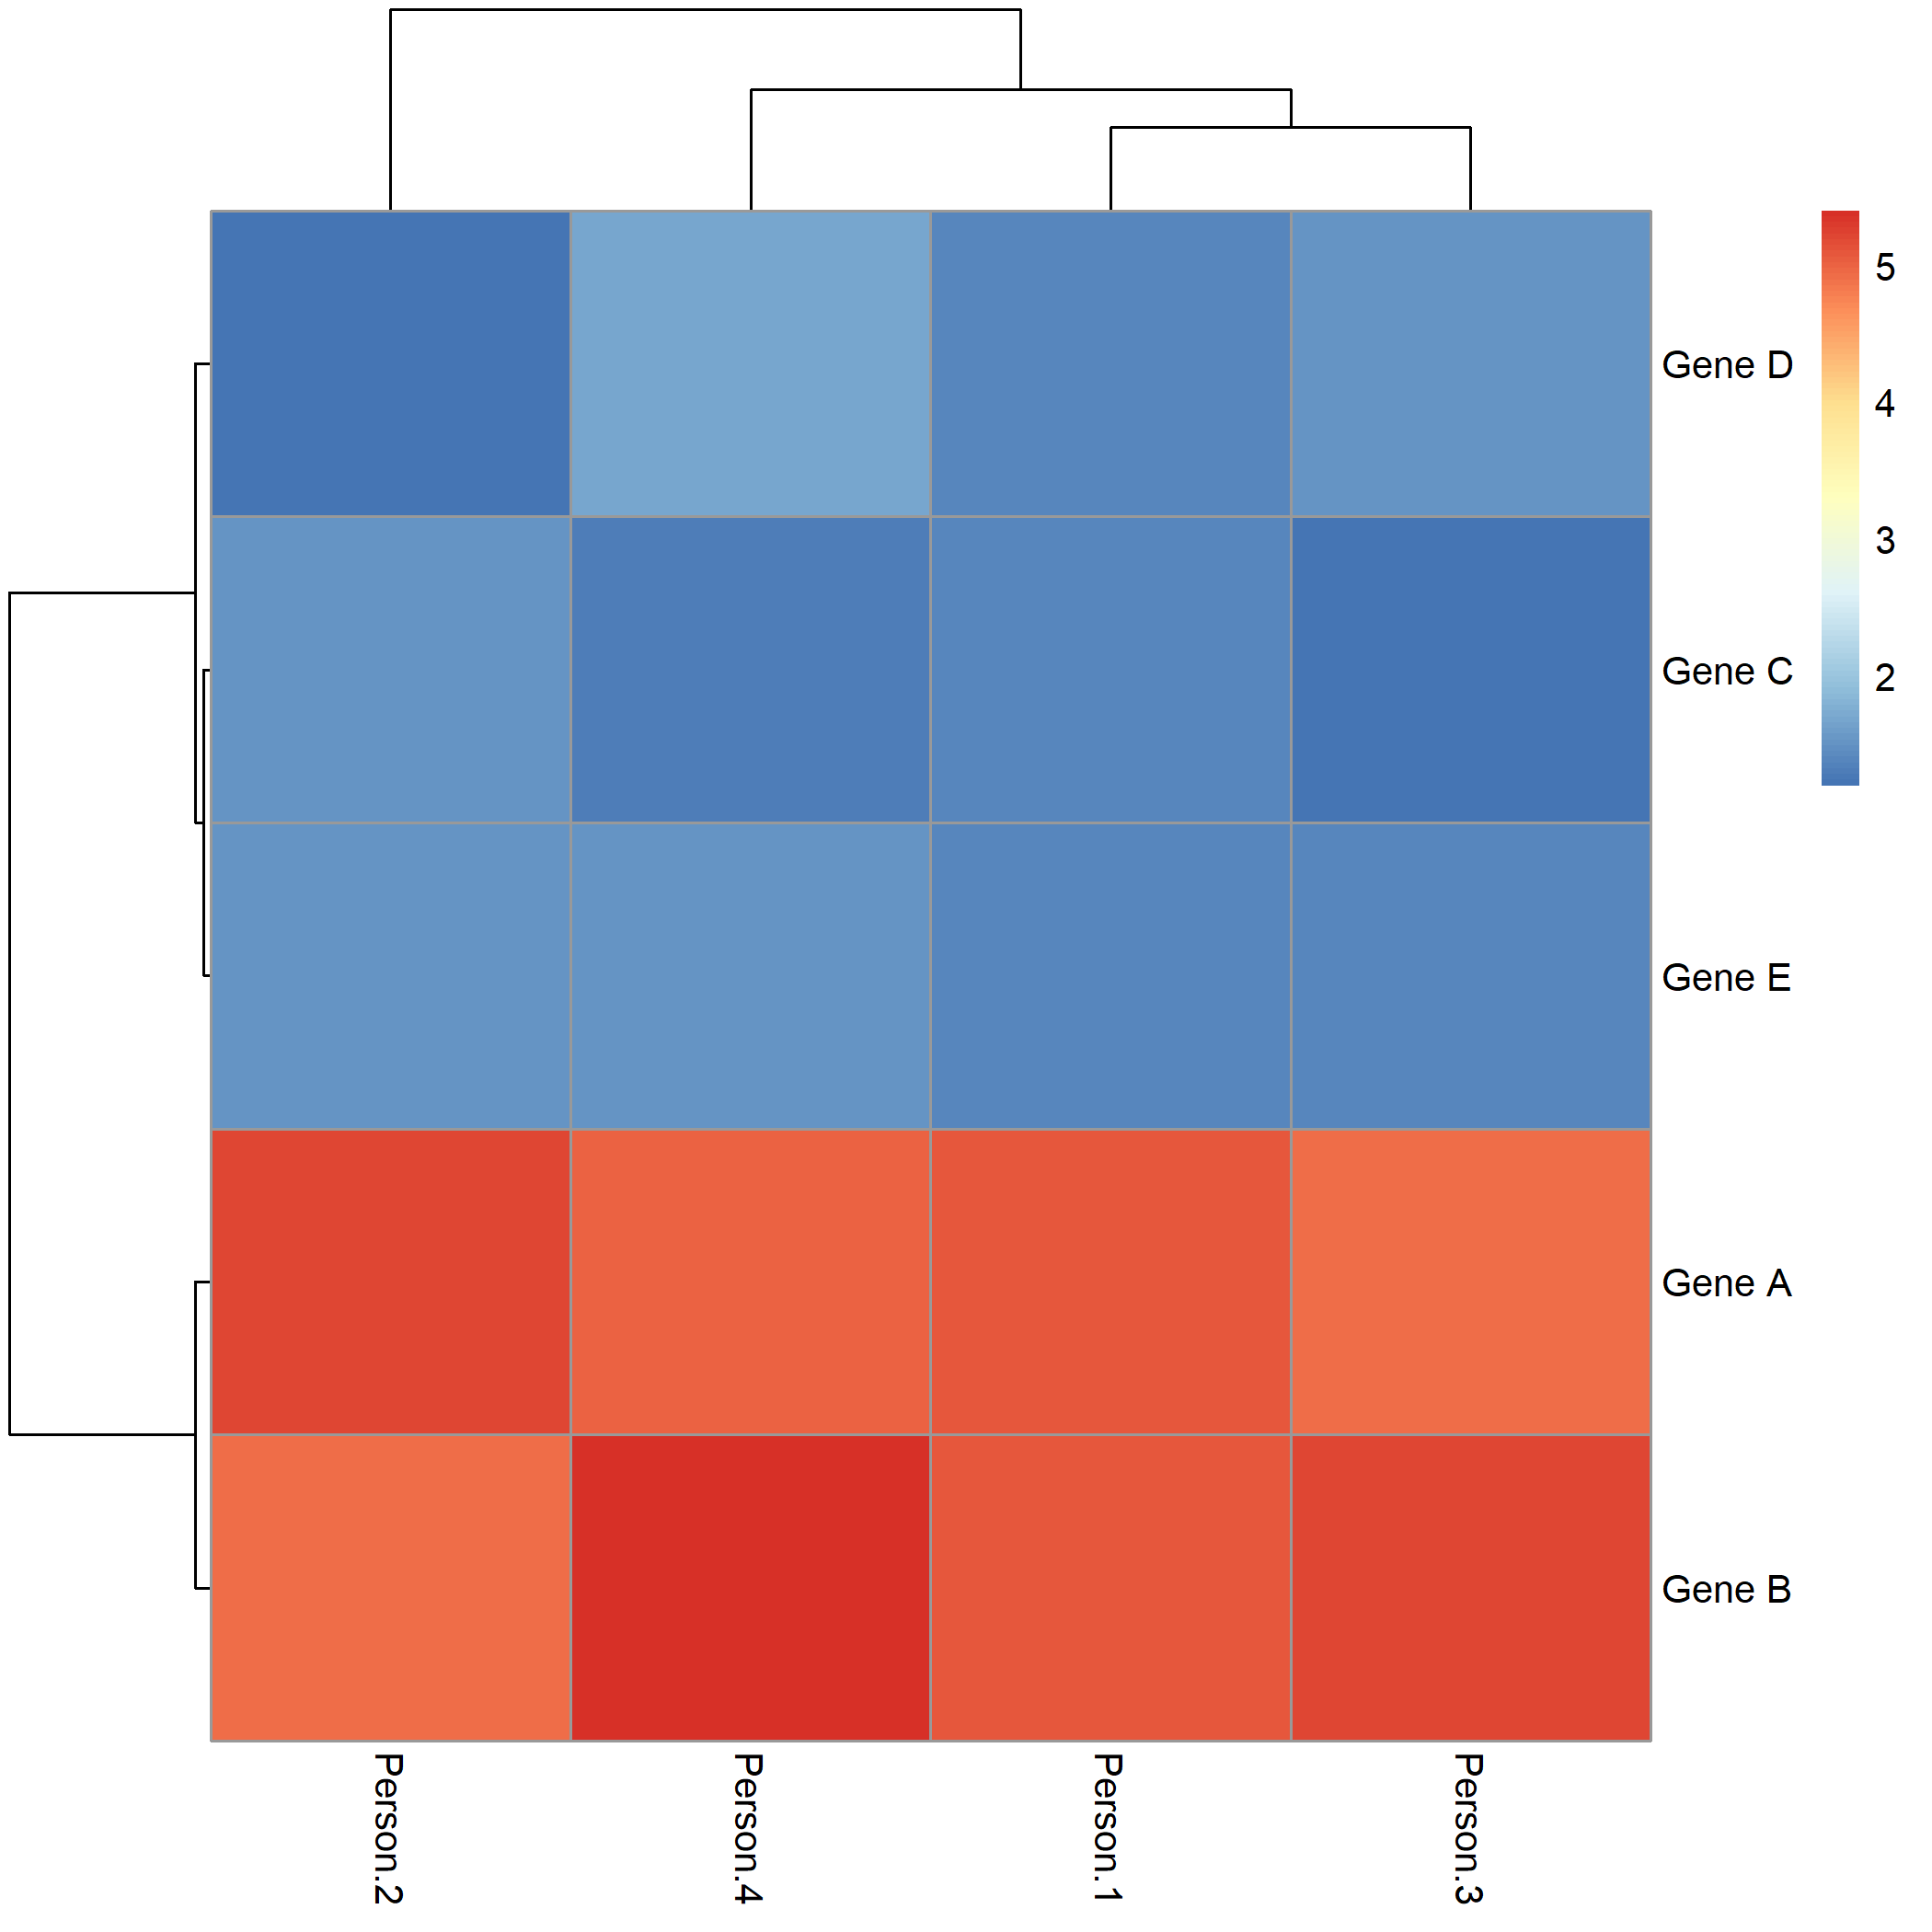
\includegraphics[scale=0.55]{Images/example_expression_data.png}
		\caption{Heatmap of expression data in table \ref{table:example_gene_expression_data} showing the clusters based upon magnitude of expression.}
		\label{fig:example_expression_data}
	\end{figure}
	One can see that genes A and C have similar patters in variation across the people, as do genes B and D. Gene E is not consistent with any other gene here. However, as this relative variation is of interest rather than the magnitude of expression, one can see that standardising the data is required. 
	
	If one were to cluster the data as represented in table \ref{table:example_gene_expression_data}, one would place genes A and B in one cluster and genes C, D and E in another as their absolute expression levels are similar (as can be seen in figure \ref{fig:example_expression_data}). However, if the expression level of each gene is standardised as per section \ref{sec:standardisation}, the data is then as represented in table \ref{table:example_standardised_gene_expression_data}. The data are now on the same scale and thus the characteristic that will determine a clustering is the variation of expression across people. As we want genes with similar patterns of variation (i.e. that are co-expressed) this enables us to cluster under our objective of defining gene sets. In this case genes A and C are one cluster, genes B and D another with gene E in a cluster alone, as can be seen in figure \ref{fig:example_standardised_expression_data}. As this is the type of data we wish to cluster across, we therefore most standardise our expression data before clustering can be implemented.
	
	\begin{table}[] 
		\centering
		\begin{tabular}{c|cccc} 
			Genes 	& Person 1	& Person 2	& Person 3	& Person 4	\\ 
			\hline
			A 		& 0.39		& 1.16 		& -1.16		& -0.39		\\
			B 		& -0.24		& -1.20		& 0.24		& 1.20		\\
			C 		& 0.39		& 1.16		& -1.16		& -0.39		\\
			D 		& -0.24		& -1.20		& 0.24		& 1.20		\\
			E 		& -0.87		& 0.87		& -0.87		& 0.87		
		\end{tabular}
		\caption{Example standardised gene expression data.}
		\label{table:example_standardised_gene_expression_data}
	\end{table}
	
	\begin{figure}[!htb]
		\centering
		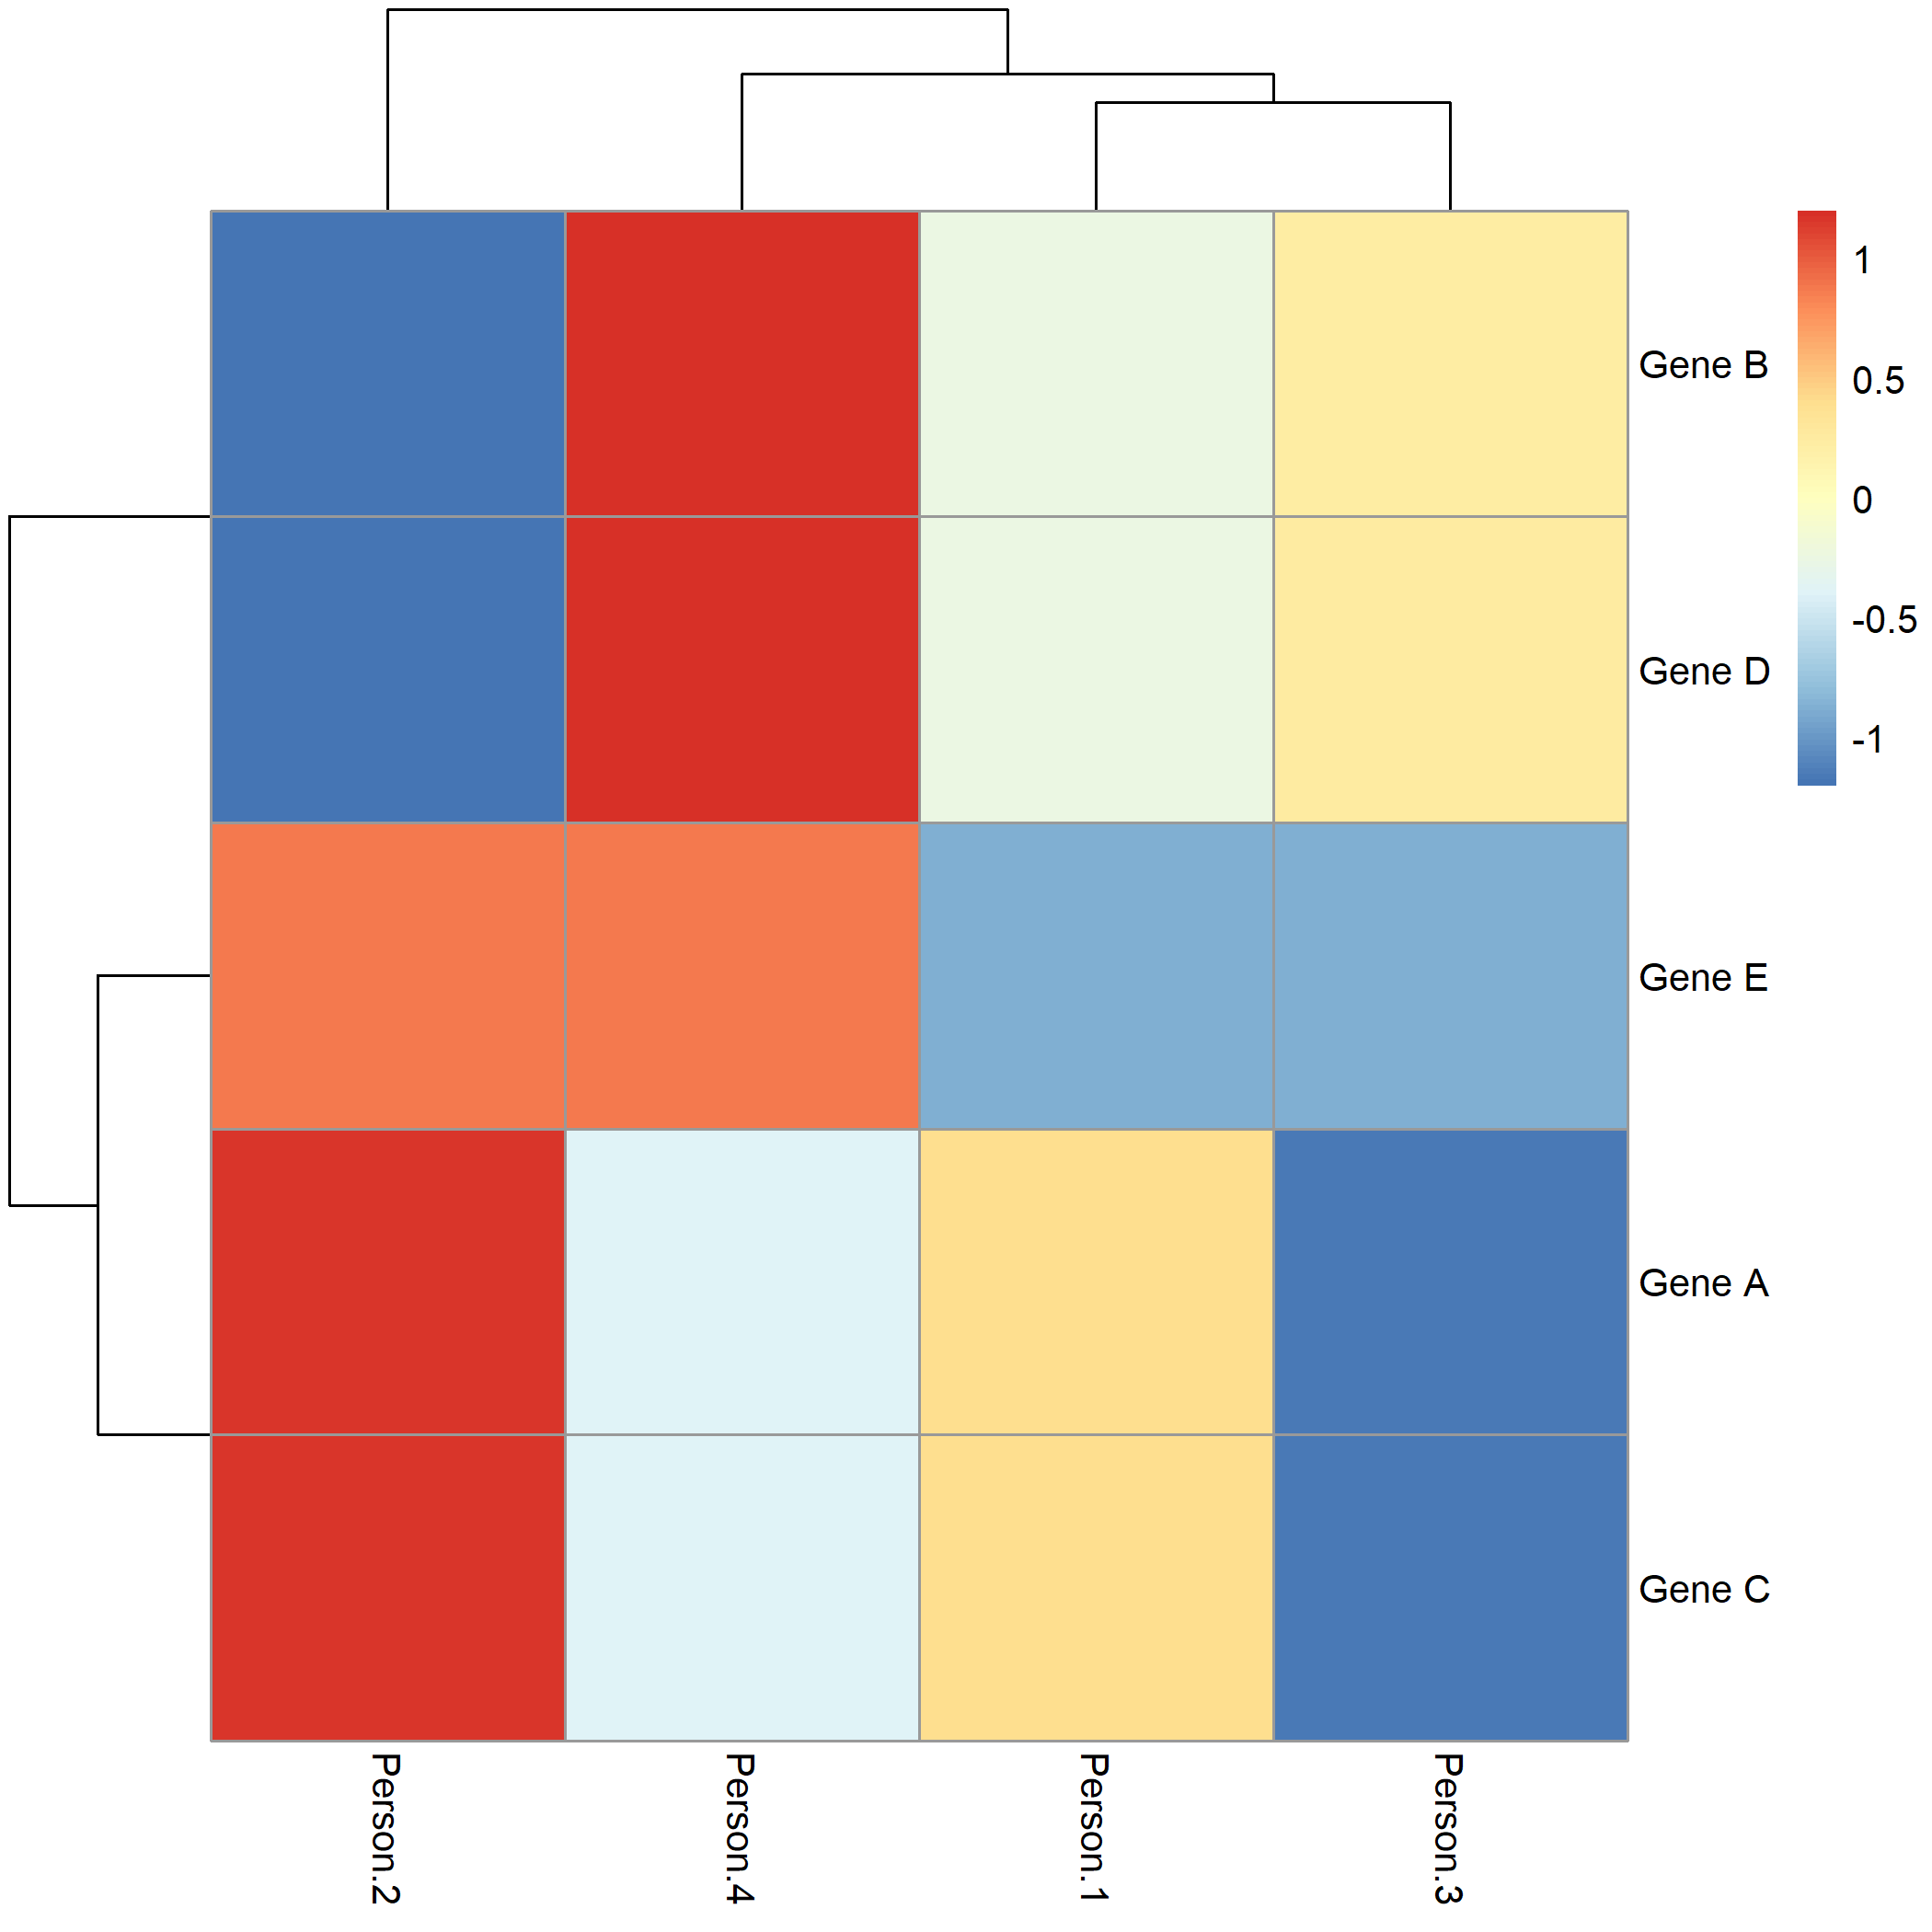
\includegraphics[scale=0.55]{Images/example_standardised_expression_data.png}
		\caption{Heatmap of expression data in table \ref{table:example_standardised_gene_expression_data} showing the clusters based upon variation of expression across people.}
		\label{fig:example_standardised_expression_data}
	\end{figure}
\end{document}